\documentclass{article}
\usepackage[utf8]{inputenc}
\usepackage{polski}
\usepackage{geometry}
\usepackage{mathabx}
\usepackage{tikz}
\usepackage{amsmath}
\usepackage{graphicx}
\usepackage{subfig}
\usepackage{amsmath}
\usepackage{hyperref}
\usepackage{pdfpages}
\usepackage{siunitx}

\geometry{
a4paper,
total={170mm,257mm},
left=20mm,
top=20mm
}
\renewcommand\thesection{}

\title{Podstawy baz danych\\ Projekt konferencje}
\author{Agnieszka Dutka, Maciek Trątnowiecki}
\date{AGH, Styczeń 2020}

\begin{document}
\maketitle
\section{Objaśnienie}
% -(1) Companies – may be – clients – każda firma ma przypisaną dokładnie 1 encję z clients (nie każdy
% klient odpowiada jakiejś firmie)
% -(2) Clients – add – participants – każdy klient może dodać wiele uczestników, każdemu uczestnikowi
% odpowiada jeden klient
% -(3) Clients – make – Conference_day_reservations - klient tworzy rezerwacje na poszczególne dni
% konferencji, relacja wiele-do-wielu
% -(4) Conference_day_registration - concerns - Conference_day_reservations - uczestnik zapisuje się
% na dany dzień konferencji na określoną rezerwację (która jest encją identyfikująca).
% -(5) Participants – take part in - Conference_day_registration - uczestnicy zapisują się na dowolną
% ilość dni koferencji, relacja wiele-do-wielu
% -(6) Participants – take part in - Workshop_registration - uczestnicy zapisują się na dowolną
% warsztatów, relacja wiele-do-wielu
% -(7) Workshop_registration - concerns - Workshop_reservations - uczestnik zapisuje się na dane
% warsztaty na określoną rezerwację (która jest encją identyfikująca).
% -(8) Clients – make – Workshop_reservations - klient tworzy rezerwacje na warsztaty, relacja wieledo-wielu
% -(9) Workshop_reservations – concerns – Workshops – na każde warsztaty mogą być dokonywane
% rezerwacje
% -(10) Workshop – is part of – Conference days – każdy warsztat ma przypisany dzień konferencji,
% relacja jeden- do-wielu
% -(11) early-signup-discounts – affects – conference_day – do dni konferencji może być przypisanych
% wiele progów cenowych
% -(12) Conference_days – is part of – Conferences – Każdy dzień konferencji należy do jakiejś
% konferencji
% -(13) Conference_day_reservations – concerns – conference_days – każda rezerwacja odnosi się do
% konkretnego dnia konferencj

        \begin{itemize}
            \item Clients - Reprezentuje klientów chcących opłacić miejsca na konferencjach i warsztatach. Klientem może być zarówno firma, jak i osoba prywatna. W zależności od tego dane klienta reprezentowane są przez odpowiednią relację w bazie. 
            
            \item Companies - Przechowuje dane klienta będącego firmą. 
            
            \item Participants - Jeżeli klient jest osobą prywatną, przechowuje jego dane. Jeżeli jest firmą, reprezentuje pojedynczego uczestnika konferencji / warsztatów. \\
            Powiązanie Clients - Participants w pierwszym przypadku występuje dokładnie raz (1..1). 
            
            % TODO: Czy to dobrze, że jest powiązany?
            W drugim każdy uczestnik konferencji powiązany jest z klientem, który opłaca jego udział w wydarzeniu (konto uczestnika tworzone jest już jako zależne od Klienta). Dzięki takiemu powiązaniu łatwo możemy sprawdzić na życzenie klienta (lub raczej działu windykacji), czy dana firma opłaciła udział wszystkich swoich pracowników. 
            
            \item Student\_id\_cards - Przechowuje informacje o legitymacjach studenckich uczestników konferencji posiadających status studenta. 
            
            \item Conferences - Reprezentuje konferencję z którą powiązane są odpowiednie dni konferencyjne, oraz warsztaty. 
            
            \item Conference\_days - Reprezentuje pojedyńczy dzień konferencji. Powiązana jest z nim ustalona opłata za uczestnictwo. Zniżki obowiązujące w zależności od daty rejestracji zwarte są w relacji Early\_Signup\_Discounts. 
            
            \item Early\_Signup\_Discounts - Odpowiada za informację o tabeli zniżek na dany dzień konferencyjny. Pojedyncza zniżka przechowywana jest w krotce z atrybutami w postaci procentowej obniżki ceny standardowej, oraz ostatniego dnia w którym obowiązuje. 
            
            \item Conference\_day\_reservations - Realizuje rezerwacje na poszczególny dzień konferencji. Każda rezerwacja powiązana jest z klientem, który ją opłaca. Za powiązanie rezerwacji z uczestnikiem odpowiada osobna relacja. Zawiera także pole due\_price określające termin płatności. Atrybut annulment\_date odpowiada za możliwość rezygnacji z podjętej rezerwacji (uznaliśmy, że usuwanie krotki z bazy może nie być optymalnym rozwiązaniem, jako że zawarte w niej dane mogą jeszcze być przydatne z punktu widzenia logiki biznesowej), w takiej sytuacji wartość null (reprezentująca brak rezygnacji - aktywność rezerwacji) zamieniane jest na datę rezygnacji. 
            
            \item Conference\_day\_registration - Wiąże rezerwację z uczestnikami konferencji. 
            
            \item Conference\_payments - Przechowuje informacje o wpływach pieniężnych powiązanych z daną rejestracją na konferencję. 
            
            \item Workshops - Reprezentuje warsztaty odbywające się w trakcie odpowiednich dni konferencyjnych. 
            
            \item Workshops\_reservations - Opisuje rezerwacje na warsztaty w sposób analogiczny do rezerwacji na konferencje. 
            
            \item Workshops\_registrations - Łączy rezerwację z uczestnikami w sposób analogiczny do dni konferencyjnyhc.
            
            \item Workshop\_payments - przechowuje informacje o wpływach pieniężnych powiązanych z daną rejestracją na warsztaty. 
        \end{itemize}
% \section{Schemat}
    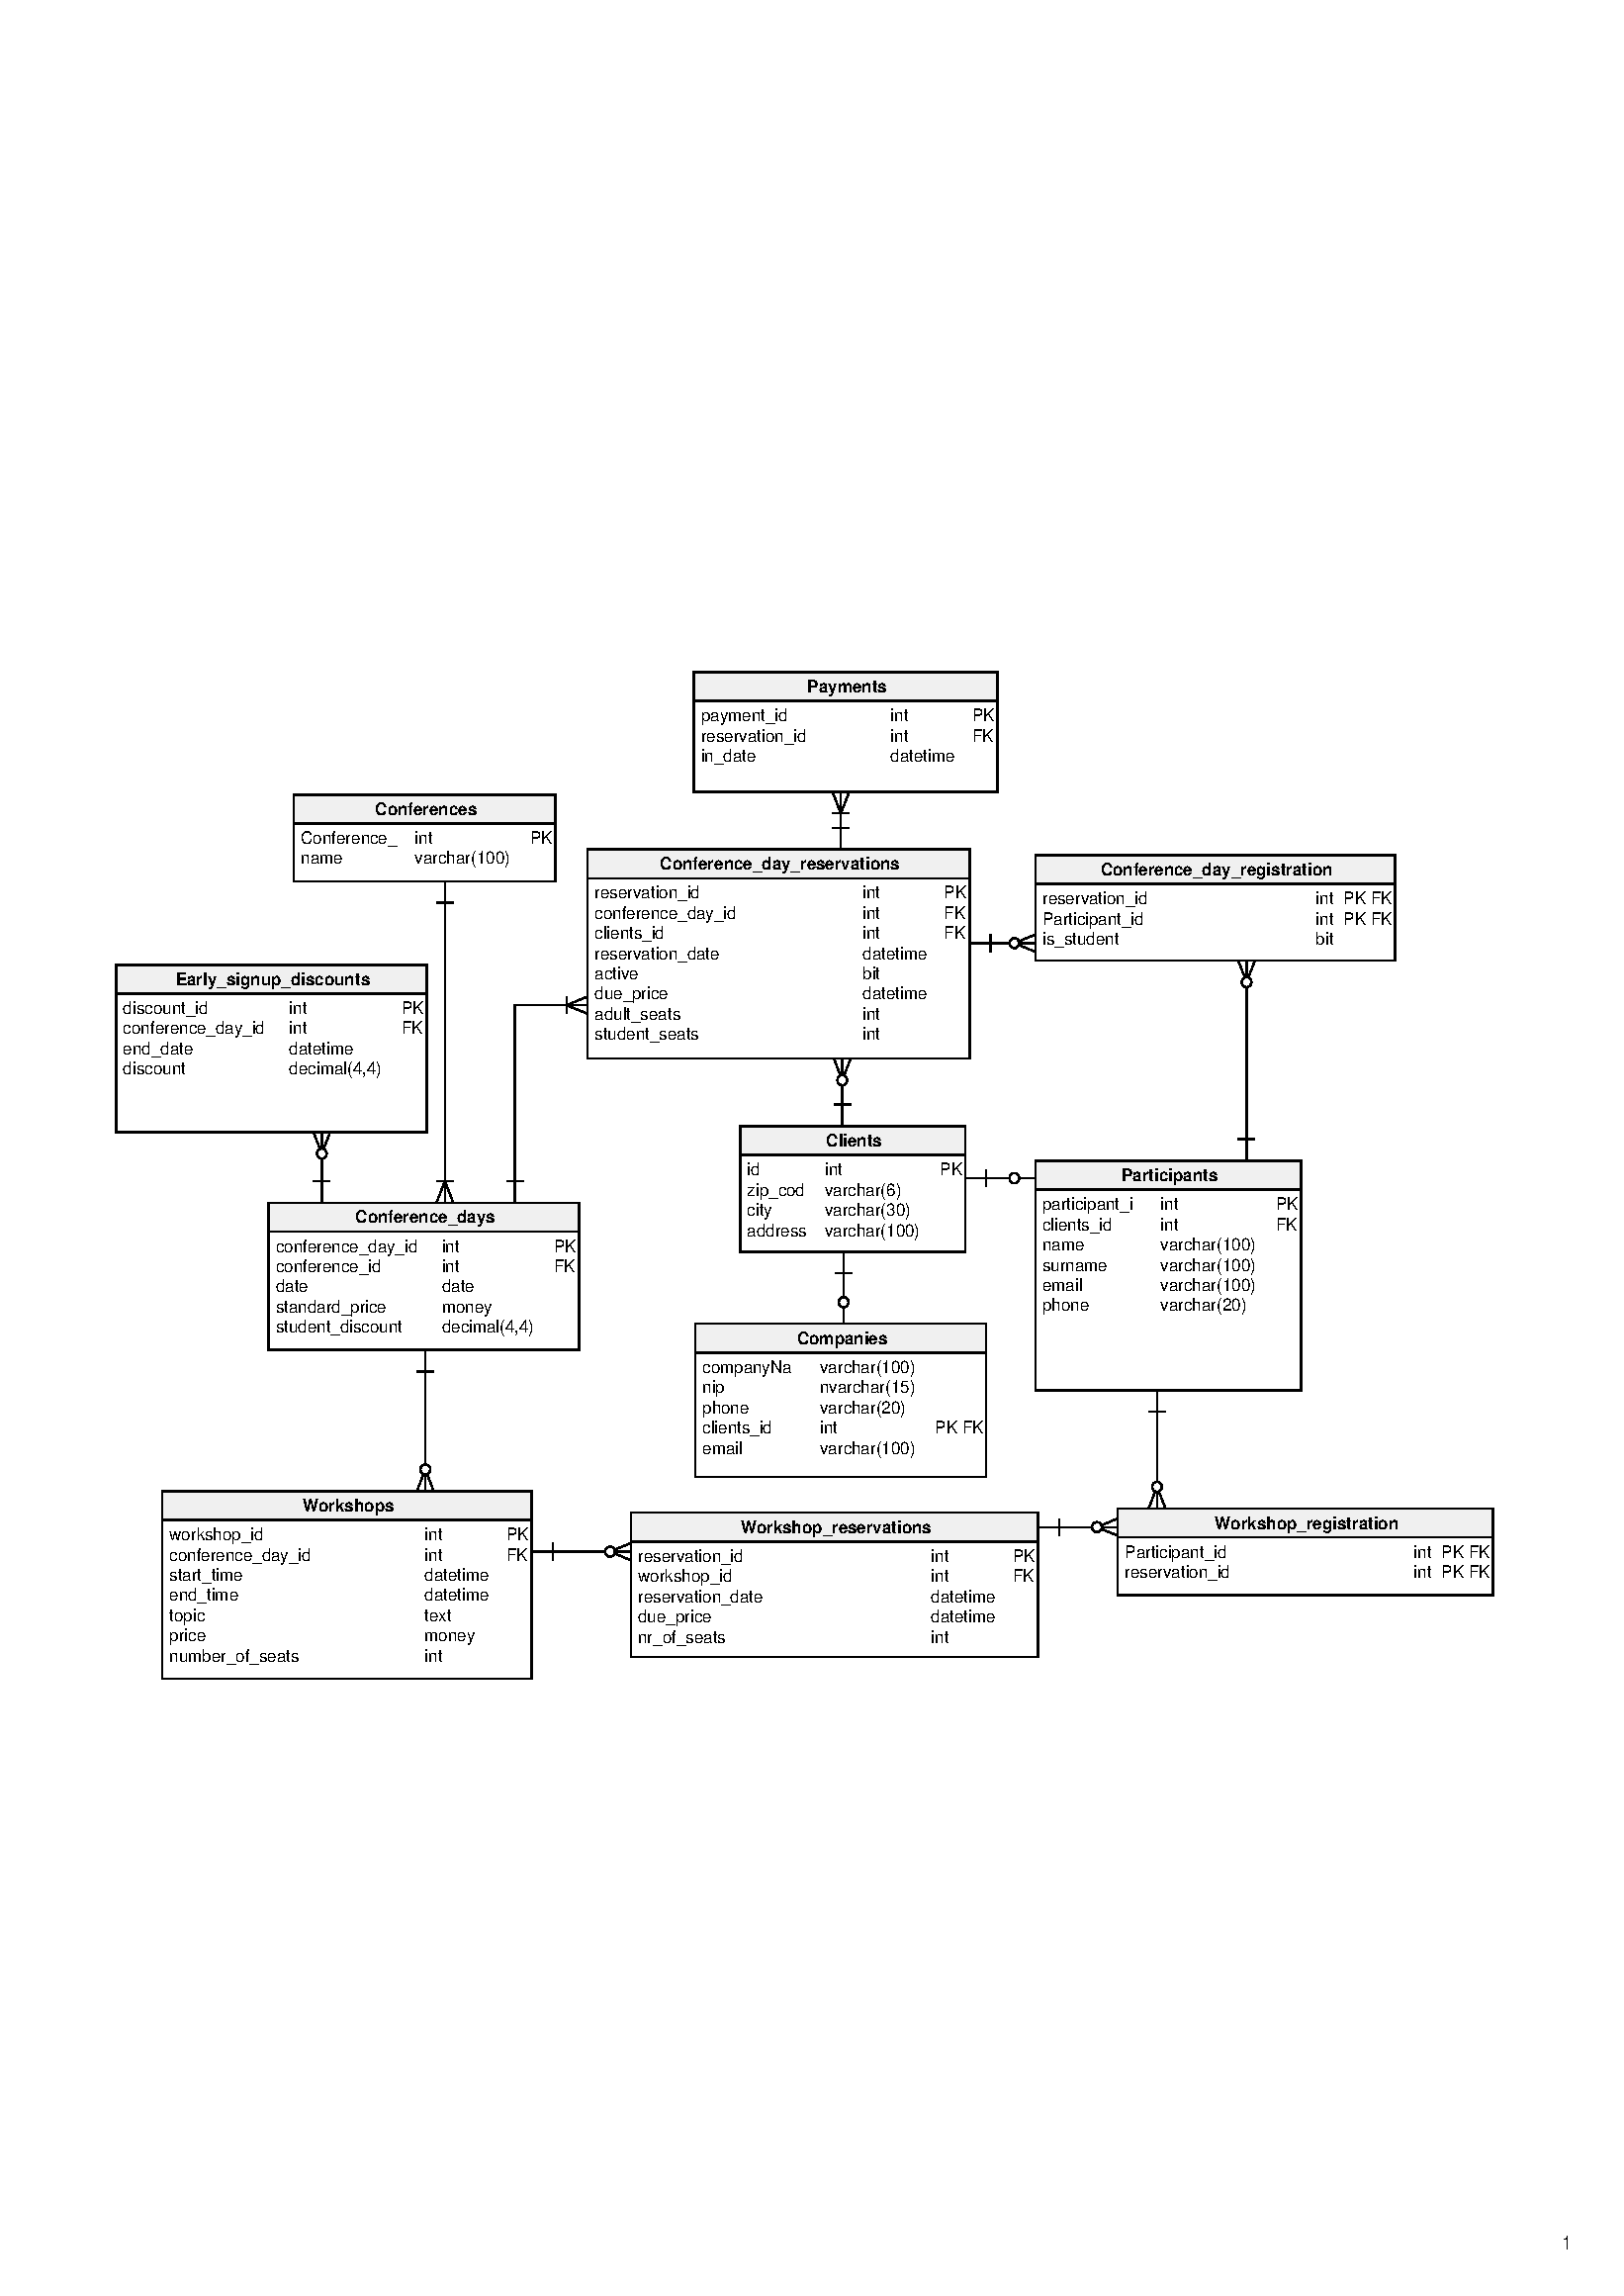
\includepdf{../Diagrams/Scheme.pdf}    

\end{document}
